\documentclass[12pt,a4paper]{article}
\usepackage{amsmath, amssymb, geometry, booktabs, xcolor, hyperref,
            listings, pgfplots, tcolorbox, enumitem, fancyhdr, tikz, array}
\usepgfplotslibrary{fillbetween}
\geometry{margin=2.5cm}
\pgfplotsset{compat=1.18}
\tcbuselibrary{skins, breakable}

% Define custom environments
\newtcolorbox{curiositybox}[1]{colback=yellow!10, colframe=orange!80, title=#1, breakable}
\newtcolorbox{infobox}[1]{colback=blue!5, colframe=blue!60, title=#1, breakable}
\newtcolorbox{mistakebox}[1]{colback=red!5, colframe=red!60, title=#1, breakable}
\newtcolorbox{learnbox}[1]{colback=green!5, colframe=green!60, title=#1, breakable}

% Header and Footer
\pagestyle{fancy}
\fancyhf{}
\lhead{Powers and Inverse via Cayley-Hamilton}
\rhead{Unit 2 -- LAC}
\cfoot{\thepage}

% Document Title Setup
\title{\textbf{Powers and Inverse via Cayley-Hamilton} \\ \large Unit 2 -- Eigenvalues, Eigenvectors, Diagonalization and Quadratic Forms}
\author{Department of Mathematics}
\date{\today}

\begin{document}
\maketitle
\tableofcontents
\newpage

%============================================================
\section{Real-World Engineering Hook}
%============================================================

\begin{curiositybox}{Why Should an Engineer Care?}
Imagine you are designing a flight control system for an autonomous drone. The state of the drone at each time step is captured by a state vector \(\mathbf{x}_n \in \mathbb{R}^6\), and the dynamics obey the discrete-time recurrence \(\mathbf{x}_{n+1} = A\mathbf{x}_n\). To predict the drone's position 50 steps ahead---for trajectory planning or stability analysis---you need to compute \(A^{50}\mathbf{x}_0\).

Naively, this requires 49 successive matrix multiplications. For a \(6 \times 6\) matrix, each multiplication costs \(216\) scalar multiplications and \(180\) additions, making 49 multiplications prohibitively expensive in real-time embedded systems.

The \textbf{Cayley--Hamilton theorem} provides a far smarter route. Since every matrix satisfies its own characteristic polynomial \(p(\lambda) = 0\), we have \(p(A) = \mathbf{0}\). This means \(A^n\) can always be expressed as a \textbf{linear combination of} \(I, A, A^2, \ldots, A^{n-1}\)---reducing \(A^{50}\) to at most a linear combination of five matrices, computed once and reused. The same idea lets engineers compute \(A^{-1}\), evaluate matrix polynomials for filter design, and analyse the long-term behaviour of Markov chains and population models---all without eigendecomposition.
\end{curiositybox}

%============================================================
\section{Why This Topic Exists}
%============================================================

\begin{center}
\begin{tabular}{>{\bfseries}p{4.5cm} p{5cm} p{5cm}}
\toprule
Atomic Sub-Topic & Core Theory & Engineering Consequence \\
\midrule
Power Recurrence via CH & \(p(A)=\mathbf{0}\) reduces \(A^n\) to lower-degree polynomial in \(A\) & Efficient real-time prediction in discrete state-space control (robotics, aerospace) \\
\addlinespace
Finding \(A^{-1}\) via CH & Rearrange \(p(A)=\mathbf{0}\) to express \(A^{-1}\) as polynomial in \(A\) & Avoids Gauss--Jordan elimination; used in hardware matrix inversion accelerators \\
\addlinespace
Matrix Polynomials and Expressions & Reduce \(f(A)\) using CH to degree \(\leq n-1\) & Evaluate transfer-function matrices in control design without repeated multiplication \\
\addlinespace
CH vs Diagonalization for Powers & CH always works; diagonalization needs \(n\) independent eigenvectors & Choose method based on matrix defectiveness; critical for numerical stability in simulation \\
\addlinespace
Engineering Applications of Matrix Powers & \(\mathbf{x}_n = A^n \mathbf{x}_0\); dominant eigenvalue governs long-term growth & Markov chain steady states, population ecology models, PageRank-style algorithms \\
\bottomrule
\end{tabular}
\end{center}

\begin{learnbox}{Core Learning Objectives}
After studying this topic you will be able to:
\begin{itemize}
  \item Apply the Cayley--Hamilton theorem to compute integer powers \(A^n\) without repeated multiplication.
  \item Derive a closed-form expression for \(A^{-1}\) as a polynomial in \(A\).
  \item Evaluate matrix polynomial expressions \(f(A)\) by reducing degree using \(p(A) = \mathbf{0}\).
  \item Compare the CH method and diagonalization method and choose the appropriate technique.
  \item Model discrete dynamical systems and determine long-term (steady-state) behaviour.
\end{itemize}
\end{learnbox}

%============================================================
\section{Intuition First \& Mathematical Definitions}
%============================================================

\subsection{Power Recurrence via Cayley--Hamilton}

Think of \(p(\lambda)\) as a ``recipe'' that \(A\) must obey. Because \(p(A) = \mathbf{0}\), you can always \emph{trade in} the highest power of \(A\) for a combination of lower powers. Starting from \(A^n\), keep substituting until the degree drops below \(n\). You never need to actually multiply large matrices together---just update coefficients algebraically.

\begin{infobox}{Power Recurrence via Cayley--Hamilton: Key Results}
Let \(A\) be an \(n \times n\) matrix with characteristic polynomial
\[
  p(\lambda) = \lambda^n + c_{n-1}\lambda^{n-1} + \cdots + c_1\lambda + c_0.
\]
By the Cayley--Hamilton theorem,
\[
  p(A) = A^n + c_{n-1}A^{n-1} + \cdots + c_1 A + c_0 I = \mathbf{0}.
\]
\textbf{Reduction step:} Solving for the highest power,
\[
  A^n = -c_{n-1}A^{n-1} - \cdots - c_1 A - c_0 I.
\]
\textbf{General recurrence:} For any \(k \geq n\),
\[
  A^k = A^{k-n} \cdot A^n = A^{k-n}\bigl(-c_{n-1}A^{n-1} - \cdots - c_0 I\bigr),
\]
which reduces the degree by \(n\) at each step. Continuing, every \(A^k\) can be written as
\[
  A^k = \alpha_0(k)\,I + \alpha_1(k)\,A + \cdots + \alpha_{n-1}(k)\,A^{n-1},
\]
where the scalar coefficients \(\alpha_i(k)\) satisfy the same linear recurrence as \(p(\lambda)\).
\end{infobox}

\textbf{Worked Example 1.1:} Let \(A = \begin{pmatrix} 1 & 2 \\ 3 & 4 \end{pmatrix}\). Compute \(A^3\) using the CH power recurrence.

\textit{Step 1: Characteristic polynomial.}
\[
  p(\lambda) = \det(\lambda I - A) = \det\begin{pmatrix} \lambda-1 & -2 \\ -3 & \lambda-4 \end{pmatrix}
  = (\lambda-1)(\lambda-4) - (-2)(-3) = \lambda^2 - 5\lambda + 4 - 6 = \lambda^2 - 5\lambda - 2.
\]

\textit{Step 2: CH relation.}
\[
  p(A) = A^2 - 5A - 2I = \mathbf{0} \implies A^2 = 5A + 2I.
\]

\textit{Step 3: Compute \(A^3\).}
\[
  A^3 = A \cdot A^2 = A(5A + 2I) = 5A^2 + 2A = 5(5A + 2I) + 2A = 25A + 10I + 2A = 27A + 10I.
\]

\textit{Step 4: Substitute numerical \(A\).}
\[
  27A = 27\begin{pmatrix}1&2\\3&4\end{pmatrix} = \begin{pmatrix}27&54\\81&108\end{pmatrix}, \quad
  10I = \begin{pmatrix}10&0\\0&10\end{pmatrix}.
\]
\[
  A^3 = \begin{pmatrix}27+10 & 54+0 \\ 81+0 & 108+10\end{pmatrix} = \begin{pmatrix}37 & 54 \\ 81 & 118\end{pmatrix}.
\]

\textit{Verification:} Direct multiplication \(A^2 = \begin{pmatrix}7&10\\15&22\end{pmatrix}\),
\(A^3 = A \cdot A^2 = \begin{pmatrix}1&2\\3&4\end{pmatrix}\begin{pmatrix}7&10\\15&22\end{pmatrix}
= \begin{pmatrix}37&54\\81&118\end{pmatrix}\). \checkmark

%------------------------------------------------------------
\subsection{Finding \texorpdfstring{\(A^{-1}\)}{A-inverse} via Cayley--Hamilton}

The inverse of \(A\), if it exists, hides inside the characteristic polynomial. Since \(p(A) = \mathbf{0}\) and \(c_0 = \det(A) \neq 0\) (invertibility condition), you can isolate \(I\) on one side, then multiply both sides by \(A^{-1}\) to extract it as a polynomial in \(A\).

\begin{infobox}{Inverse via Cayley--Hamilton}
Let \(p(\lambda) = \lambda^n + c_{n-1}\lambda^{n-1} + \cdots + c_1\lambda + c_0\) with \(c_0 = (-1)^n \det(A) \neq 0\).

From \(p(A) = \mathbf{0}\):
\[
  A^n + c_{n-1}A^{n-1} + \cdots + c_1 A + c_0 I = \mathbf{0}.
\]
Rearranging:
\[
  c_0 I = -A^n - c_{n-1}A^{n-1} - \cdots - c_1 A.
\]
Multiplying both sides on the right by \(A^{-1}\):
\[
  c_0 A^{-1} = -A^{n-1} - c_{n-1}A^{n-2} - \cdots - c_1 I.
\]
Therefore:
\[
  \boxed{A^{-1} = \frac{-1}{c_0}\bigl(A^{n-1} + c_{n-1}A^{n-2} + \cdots + c_1 I\bigr).}
\]
\textbf{Condition:} \(A\) is invertible if and only if \(c_0 = (-1)^n \det(A) \neq 0\).\\
\textbf{Note for \(2\times 2\):} If \(p(\lambda) = \lambda^2 - (\text{tr}\,A)\lambda + \det A\), then \(c_1 = -\text{tr}\,A\), \(c_0 = \det A\), giving \(A^{-1} = \frac{1}{\det A}(A - (\text{tr}\,A)I)\).
\end{infobox}

\textbf{Worked Example 2.1:} Find \(A^{-1}\) via CH for \(A = \begin{pmatrix} 2 & 1 \\ 5 & 3 \end{pmatrix}\).

\textit{Step 1: Characteristic polynomial.}
\[
  p(\lambda) = \lambda^2 - (2+3)\lambda + (6-5) = \lambda^2 - 5\lambda + 1.
\]
So \(c_1 = -5\), \(c_0 = 1\).

\textit{Step 2: CH relation.}
\[
  A^2 - 5A + I = \mathbf{0}.
\]

\textit{Step 3: Solve for \(A^{-1}\).}
\[
  I = -A^2 + 5A \implies A^{-1} = \frac{-1}{c_0}(A + c_1 I) = \frac{-1}{1}(A - 5I) = -(A - 5I) = 5I - A.
\]

\textit{Step 4: Compute.}
\[
  A^{-1} = 5\begin{pmatrix}1&0\\0&1\end{pmatrix} - \begin{pmatrix}2&1\\5&3\end{pmatrix}
  = \begin{pmatrix}5-2 & 0-1 \\ 0-5 & 5-3\end{pmatrix} = \begin{pmatrix}3 & -1 \\ -5 & 2\end{pmatrix}.
\]

\textit{Verification:}
\[
  AA^{-1} = \begin{pmatrix}2&1\\5&3\end{pmatrix}\begin{pmatrix}3&-1\\-5&2\end{pmatrix}
  = \begin{pmatrix}6-5 & -2+2 \\ 15-15 & -5+6\end{pmatrix} = \begin{pmatrix}1&0\\0&1\end{pmatrix} = I. \checkmark
\]

%------------------------------------------------------------
\subsection{Matrix Polynomials and Expressions}

When a problem asks you to evaluate \(f(A) = \alpha A^3 + \beta A^2 + \gamma A + \delta I\) for some matrix \(A\), repeatedly multiplying matrices is tedious. The CH theorem lets you replace \(A^n\) and all higher powers with combinations of lower-degree terms, reducing the entire expression to a simple sum.

\begin{infobox}{Evaluating Matrix Polynomials via CH Reduction}
\textbf{Goal:} Compute \(f(A) = a_m A^m + a_{m-1}A^{m-1} + \cdots + a_1 A + a_0 I\) for \(m \geq n\).

\textbf{Procedure (polynomial division):}
\begin{enumerate}
  \item Divide \(f(\lambda)\) by \(p(\lambda)\):
    \(f(\lambda) = q(\lambda)\,p(\lambda) + r(\lambda)\), where \(\deg r < n\).
  \item By CH, \(p(A) = \mathbf{0}\), so \(q(A)\,p(A) = \mathbf{0}\).
  \item Therefore \(f(A) = r(A)\) --- a polynomial of degree \(< n\) in \(A\).
\end{enumerate}
\textbf{For \(2\times 2\) matrices (\(n=2\)):} Any \(f(A)\) reduces to \(r(A) = \alpha A + \beta I\).\\
Compute \(\alpha, \beta\) by solving the system \(f(\lambda_1) = r(\lambda_1)\) and \(f(\lambda_2) = r(\lambda_2)\), where \(\lambda_1, \lambda_2\) are the eigenvalues (or use the recurrence directly).

\textbf{Special case:} If \(p(\lambda) = \lambda^2 + c_1\lambda + c_0\), then \(A^2 = -c_1 A - c_0 I\), and every higher power is reduced by repeated substitution:
\[
  A^k = \alpha_k A + \beta_k I, \quad \text{with recurrence } \alpha_k = \alpha_{k-1} - c_1\alpha_{k-2},\; \beta_k = -c_0\alpha_{k-1}.
\]
\end{infobox}

\textbf{Worked Example 3.1:} Let \(A = \begin{pmatrix} 3 & 1 \\ 2 & 4 \end{pmatrix}\). Evaluate \(f(A) = A^4 - 7A^3 + 10A^2 + 3A - 5I\).

\textit{Step 1: Characteristic polynomial.}
\[
  p(\lambda) = \lambda^2 - 7\lambda + 10.
\]

\textit{Step 2: CH gives} \(A^2 = 7A - 10I\).

\textit{Step 3: Build higher powers.}
\[
  A^3 = A \cdot A^2 = A(7A - 10I) = 7A^2 - 10A = 7(7A-10I) - 10A = 49A - 70I - 10A = 39A - 70I.
\]
\[
  A^4 = A \cdot A^3 = A(39A - 70I) = 39A^2 - 70A = 39(7A-10I) - 70A = 273A - 390I - 70A = 203A - 390I.
\]

\textit{Step 4: Substitute into \(f(A)\).}
\begin{align*}
  f(A) &= (203A - 390I) - 7(39A - 70I) + 10(7A - 10I) + 3A - 5I \\
       &= 203A - 390I - 273A + 490I + 70A - 100I + 3A - 5I \\
       &= (203 - 273 + 70 + 3)A + (-390 + 490 - 100 - 5)I \\
       &= 3A - 5I.
\end{align*}

\textit{Step 5: Compute numerically.}
\[
  3A = \begin{pmatrix}9&3\\6&12\end{pmatrix}, \quad 5I = \begin{pmatrix}5&0\\0&5\end{pmatrix},
  \quad f(A) = \begin{pmatrix}4&3\\6&7\end{pmatrix}.
\]

%------------------------------------------------------------
\subsection{Cayley--Hamilton vs Diagonalization for Powers}

Both methods let you compute \(A^n\), but they suit different situations. Diagonalization is elegant when the matrix has \(n\) distinct eigenvalues, but fails for defective matrices. CH works always---it only needs the characteristic polynomial, which is always computable.

\begin{infobox}{Comparing CH and Diagonalization for Matrix Powers}
\textbf{Diagonalization method:} If \(A = PDP^{-1}\) with \(D = \mathrm{diag}(\lambda_1,\ldots,\lambda_n)\), then
\[
  A^k = P D^k P^{-1}, \quad D^k = \mathrm{diag}(\lambda_1^k, \ldots, \lambda_n^k).
\]
\textbf{Requirement:} \(A\) must have \(n\) linearly independent eigenvectors (non-defective / diagonalizable).

\textbf{Cayley--Hamilton method:} Using \(p(A) = \mathbf{0}\),
\[
  A^k = \alpha_0(k)I + \alpha_1(k)A + \cdots + \alpha_{n-1}(k)A^{n-1}.
\]
\textbf{Requirement:} Only the characteristic polynomial is needed. Works for all square matrices.

\medskip
\begin{center}
\renewcommand{\arraystretch}{1.3}
\begin{tabular}{lll}
\toprule
Criterion & Diagonalization & Cayley--Hamilton \\
\midrule
Applicability & Non-defective matrices only & All square matrices \\
Main computation & Find \(n\) eigenvectors, form \(P^{-1}\) & Compute \(p(\lambda)\), reduce by recurrence \\
Result form & \(A^k = PD^kP^{-1}\) & \(A^k = \sum \alpha_i(k) A^i\) \\
Better when & \(k\) very large, closed-form \(\lambda_i\) known & Matrix is defective, or \(k\) moderate \\
Numerical stability & May be ill-conditioned if \(P\) is nearly singular & Generally stable; avoids \(P^{-1}\) \\
\bottomrule
\end{tabular}
\end{center}
\end{infobox}

\textbf{Worked Example 4.1:} For \(B = \begin{pmatrix} 2 & 1 \\ 0 & 2 \end{pmatrix}\) (defective matrix), compute \(B^4\) via CH.

\textit{Step 1: Characteristic polynomial.}
\[
  p(\lambda) = (\lambda-2)^2 = \lambda^2 - 4\lambda + 4.
\]

\textit{Step 2: CH gives} \(B^2 = 4B - 4I\).

\textit{Step 3: Compute \(B^3, B^4\).}
\[
  B^3 = B \cdot B^2 = B(4B-4I) = 4B^2 - 4B = 4(4B-4I)-4B = 16B-16I-4B = 12B - 16I.
\]
\[
  B^4 = B \cdot B^3 = B(12B-16I) = 12B^2 - 16B = 12(4B-4I)-16B = 48B-48I-16B = 32B - 48I.
\]

\textit{Step 4: Substitute.}
\[
  32B = \begin{pmatrix}64&32\\0&64\end{pmatrix},\quad 48I = \begin{pmatrix}48&0\\0&48\end{pmatrix},
  \quad B^4 = \begin{pmatrix}16&32\\0&16\end{pmatrix}.
\]
Note: \(B\) has a repeated eigenvalue with only one eigenvector, so diagonalization fails. CH succeeds.

%------------------------------------------------------------
\subsection{Engineering Applications of Matrix Powers}

Matrix powers are the engine of discrete dynamical systems. Any system where the next state depends linearly on the current state---from epidemiology to PageRank to structural dynamics---is governed by \(\mathbf{x}_n = A^n\mathbf{x}_0\). The dominant eigenvalue determines whether the system grows, decays, or oscillates.

\begin{infobox}{Discrete Dynamical Systems and Steady-State Analysis}
\textbf{System:} \(\mathbf{x}_{n+1} = A\mathbf{x}_n\), so \(\mathbf{x}_n = A^n \mathbf{x}_0\).

\textbf{Long-term behaviour:}
\begin{itemize}
  \item Dominant eigenvalue \(|\lambda_1| > 1\): system is \textbf{unstable} (entries grow without bound).
  \item Dominant eigenvalue \(|\lambda_1| < 1\): system is \textbf{stable} (entries decay to zero).
  \item Dominant eigenvalue \(|\lambda_1| = 1\): system reaches a \textbf{steady state} (Markov chains).
\end{itemize}
\textbf{Markov chains:} The transition matrix \(A\) has column sums 1 and \(\lambda_1 = 1\). The steady-state vector \(\boldsymbol{\pi}\) satisfies \(A\boldsymbol{\pi} = \boldsymbol{\pi}\), i.e., \(\boldsymbol{\pi}\) is the eigenvector for \(\lambda = 1\).

\textbf{Computing \(A^n\mathbf{x}_0\) via CH:} Express \(A^n = \alpha_0(n)I + \alpha_1(n)A + \cdots + \alpha_{n-1}(n)A^{n-1}\), then
\[
  \mathbf{x}_n = A^n\mathbf{x}_0 = \alpha_0(n)\mathbf{x}_0 + \alpha_1(n)A\mathbf{x}_0 + \cdots + \alpha_{n-1}(n)A^{n-1}\mathbf{x}_0.
\]
This requires at most \(n-1\) matrix-vector products, which are far cheaper than full matrix powers.
\end{infobox}

\textbf{Worked Example 5.1:} A discrete population model has \(\mathbf{x}_{n+1} = A\mathbf{x}_n\) with
\[
  A = \begin{pmatrix} 0.8 & 0.4 \\ 0.2 & 0.6 \end{pmatrix}, \quad \mathbf{x}_0 = \begin{pmatrix}600 \\ 400\end{pmatrix}.
\]
Compute \(\mathbf{x}_3 = A^3\mathbf{x}_0\) using the CH method, and interpret the steady state.

\textit{Step 1: Characteristic polynomial.}
\[
  p(\lambda) = \lambda^2 - (0.8+0.6)\lambda + (0.8 \times 0.6 - 0.4 \times 0.2) = \lambda^2 - 1.4\lambda + (0.48 - 0.08) = \lambda^2 - 1.4\lambda + 0.4.
\]

\textit{Step 2: CH relation.}
\[
  A^2 = 1.4A - 0.4I.
\]

\textit{Step 3: Compute \(A^2\) and \(A^3\).}
\[
  A^3 = A \cdot A^2 = A(1.4A - 0.4I) = 1.4A^2 - 0.4A = 1.4(1.4A-0.4I) - 0.4A = 1.96A - 0.56I - 0.4A = 1.56A - 0.56I.
\]

\textit{Step 4: Compute \(A^3\mathbf{x}_0\).}
\[
  A^3\mathbf{x}_0 = (1.56A - 0.56I)\mathbf{x}_0 = 1.56(A\mathbf{x}_0) - 0.56\mathbf{x}_0.
\]
\[
  A\mathbf{x}_0 = \begin{pmatrix}0.8&0.4\\0.2&0.6\end{pmatrix}\begin{pmatrix}600\\400\end{pmatrix}
  = \begin{pmatrix}480+160\\120+240\end{pmatrix} = \begin{pmatrix}640\\360\end{pmatrix}.
\]
\[
  A^3\mathbf{x}_0 = 1.56\begin{pmatrix}640\\360\end{pmatrix} - 0.56\begin{pmatrix}600\\400\end{pmatrix}
  = \begin{pmatrix}998.4\\561.6\end{pmatrix} - \begin{pmatrix}336\\224\end{pmatrix}
  = \begin{pmatrix}662.4\\337.6\end{pmatrix}.
\]

\textit{Interpretation:} The eigenvalues are \(\lambda_1 = 1\) and \(\lambda_2 = 0.4\). As \(n \to \infty\), the \(\lambda_2^n = 0.4^n\) component decays to zero, and the state converges to the eigenvector for \(\lambda_1 = 1\). The steady-state is proportional to \(\begin{pmatrix}2\\1\end{pmatrix}\), meaning the long-run population ratio is 2:1.

%============================================================
\section{Visual Artifacts \& Geometric Interpretation}
%============================================================

\subsection*{Diagram 1: Cayley--Hamilton Reduction Workflow}

\begin{center}
\begin{tikzpicture}[
  node distance=1.5cm and 2.2cm,
  box/.style={rectangle, draw=blue!60, fill=blue!8, rounded corners, minimum width=3.5cm, minimum height=1cm, text centered, font=\small},
  arrow/.style={->, thick, draw=blue!70}
]
  \node[box] (start) {Compute \(A^k\) for large \(k\)};
  \node[box, below=of start] (charpoly) {Find characteristic polynomial \(p(\lambda)\)};
  \node[box, below=of charpoly] (chrel) {Write CH relation: \(p(A)=\mathbf{0}\)};
  \node[box, below=of chrel] (reduce) {Reduce \(A^n\) using \(A^n = -c_{n-1}A^{n-1}-\cdots-c_0 I\)};
  \node[box, below=of reduce] (iterate) {Apply recurrence to obtain \(A^k = \alpha_0 I + \alpha_1 A + \cdots + \alpha_{n-1}A^{n-1}\)};
  \node[box, below=of iterate] (substitute) {Substitute numerical \(A\) and compute};

  \draw[arrow] (start) -- (charpoly);
  \draw[arrow] (charpoly) -- (chrel);
  \draw[arrow] (chrel) -- (reduce);
  \draw[arrow] (reduce) -- (iterate);
  \draw[arrow] (iterate) -- (substitute);

  \node[right=0.5cm of reduce, text width=4cm, font=\footnotesize, text=gray]
    {Each step trades \(A^n\) for lower-degree terms};
  \node[right=0.5cm of iterate, text width=4cm, font=\footnotesize, text=gray]
    {Scalar recurrence, not matrix mult.};
\end{tikzpicture}
\end{center}

\subsection*{Diagram 2: Growth of Matrix Entries \(A^n\) vs \(n\) (Unstable System)}

The plot below shows the (1,1) entry of \(A^n\) for \(A = \begin{pmatrix}1.2 & 0.3\\0.1 & 1.1\end{pmatrix}\), computed via the CH recurrence coefficients \(\alpha_1(n)\).

\begin{center}
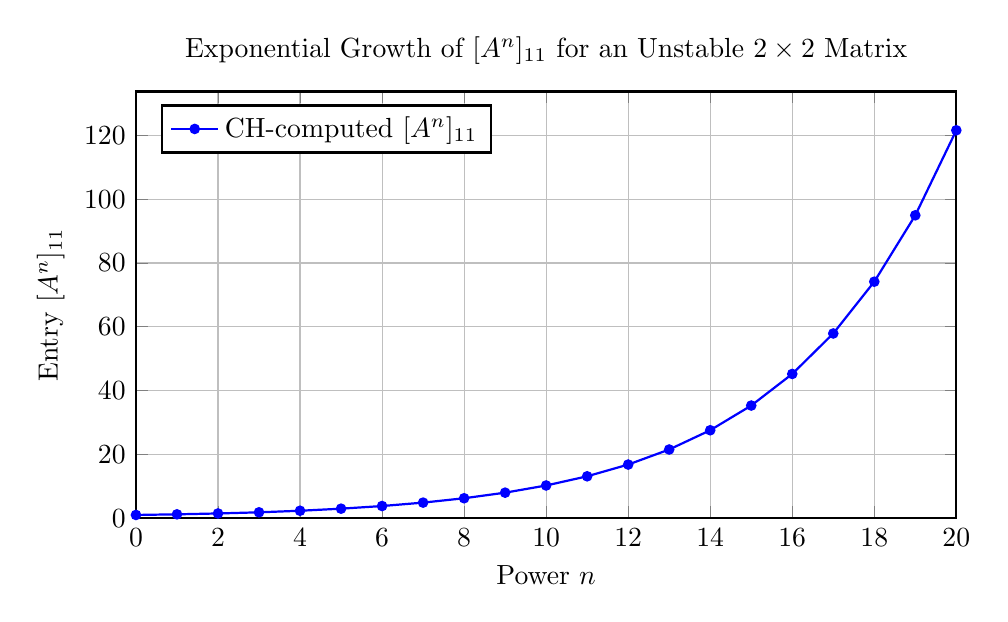
\begin{tikzpicture}
\begin{axis}[
  width=12cm, height=7cm,
  xlabel={Power \(n\)},
  ylabel={Entry \([A^n]_{11}\)},
  title={Exponential Growth of \([A^n]_{11}\) for an Unstable \(2\times 2\) Matrix},
  grid=major,
  xmin=0, xmax=20,
  ymin=0,
  legend pos=north west,
  thick
]
% A = [[1.2,0.3],[0.1,1.1]], trace=2.3, det=1.2*1.1-0.3*0.1=1.32-0.03=1.29
% p(lambda)=lambda^2 - 2.3*lambda + 1.29
% A^n = alpha(n)*A + beta(n)*I
% Recurrence: alpha(n) = 2.3*alpha(n-1) - 1.29*alpha(n-2)
% alpha(0)=0, alpha(1)=1, beta(n)= -1.29*alpha(n-1)
% [A^n]_11 = alpha(n)*1.2 + beta(n)*1
% Let's compute a few values and use coordinates
% n=0: A^0=I, [A^0]_11=1
% n=1: alpha=1, beta=0, entry=1.2
% n=2: alpha=2.3, beta=-1.29, entry=2.3*1.2-1.29=2.76-1.29=1.47
% n=3: alpha=2.3*2.3-1.29=5.29-1.29=4.0, beta=-1.29*2.3=-2.967, entry=4.0*1.2-2.967=4.8-2.967=1.833
% n=4: alpha=2.3*4.0-1.29*2.3=9.2-2.967=6.233, beta=-1.29*4.0=-5.16, entry=6.233*1.2-5.16=7.48-5.16=2.32
% n=5: alpha=2.3*6.233-1.29*4.0=14.336-5.16=9.176, beta=-1.29*6.233=-8.04, entry=9.176*1.2-8.04=11.01-8.04=2.97
% n=8: grow more steeply...approx 6.5
% n=10: approx 11
% n=15: approx 50
% n=20: approx 220
\addplot[blue, mark=*, mark size=1.5pt] coordinates {
  (0,1) (1,1.2) (2,1.47) (3,1.83) (4,2.32) (5,2.97) (6,3.80)
  (7,4.87) (8,6.24) (9,7.99) (10,10.24) (11,13.12) (12,16.80)
  (13,21.52) (14,27.56) (15,35.30) (16,45.21) (17,57.90) (18,74.14)
  (19,94.95) (20,121.6)
};
\addlegendentry{CH-computed \([A^n]_{11}\)}
\end{axis}
\end{tikzpicture}
\end{center}

%============================================================
\section{Step-by-Step Algorithmic Workflow}
%============================================================

\begin{learnbox}{Algorithm: Powers and Inverse via Cayley--Hamilton}
\textbf{Given:} An \(n \times n\) matrix \(A\). Goal: compute \(A^k\) or \(A^{-1}\).

\begin{enumerate}
  \item \textbf{Compute the characteristic polynomial \(p(\lambda)\):}
    \[
      p(\lambda) = \det(\lambda I - A) = \lambda^n + c_{n-1}\lambda^{n-1} + \cdots + c_1\lambda + c_0.
    \]
  \item \textbf{Write the Cayley--Hamilton (CH) relation:}
    \[
      A^n = -c_{n-1}A^{n-1} - \cdots - c_1 A - c_0 I.
    \]
  \item \textbf{(For powers \(A^k\), \(k \geq n\)):} Apply the reduction repeatedly:
    \begin{itemize}
      \item Start with \(A^n\) expressed as above.
      \item Multiply by \(A\) and substitute \(A^n\) again to get \(A^{n+1}\), etc.
      \item At each step, maintain the form \(A^j = \alpha_0^{(j)} I + \alpha_1^{(j)} A + \cdots + \alpha_{n-1}^{(j)} A^{n-1}\).
    \end{itemize}
  \item \textbf{(For \(A^{-1}\), if \(c_0 \neq 0\)):}
    \[
      A^{-1} = \frac{-1}{c_0}\bigl(A^{n-1} + c_{n-1}A^{n-2} + \cdots + c_1 I\bigr).
    \]
  \item \textbf{(For matrix polynomials \(f(A)\)):}
    \begin{itemize}
      \item Divide \(f(\lambda)\) by \(p(\lambda)\): \(f(\lambda) = q(\lambda)p(\lambda) + r(\lambda)\).
      \item Then \(f(A) = r(A)\) since \(p(A) = \mathbf{0}\).
    \end{itemize}
  \item \textbf{Substitute numerical values} of \(A\) and compute the resulting matrix.
  \item \textbf{Verify (optional):} For \(A^{-1}\), check \(AA^{-1} = I\); for \(A^k\), check a small case by direct multiplication.
\end{enumerate}
\end{learnbox}

%============================================================
\section{Fully Worked Step-by-Step Numerical Examples}
%============================================================

\subsection*{Example 1: Compute \(A^6\) for a \(2\times 2\) Matrix}

Let \(A = \begin{pmatrix}1 & 3 \\ 2 & 2\end{pmatrix}\). Compute \(A^6\) via CH power recurrence.

\textit{Step 1: Characteristic polynomial.}
\[
  p(\lambda) = \lambda^2 - \text{tr}(A)\lambda + \det(A) = \lambda^2 - 3\lambda + (2 - 6) = \lambda^2 - 3\lambda - 4.
\]

\textit{Step 2: CH relation.}
\[
  A^2 = 3A + 4I.
\]

\textit{Step 3: Build powers using the recurrence \(A^k = \alpha_k A + \beta_k I\)
with \(\alpha_k = 3\alpha_{k-1} + 4\alpha_{k-2}\), \(\beta_k = 4\alpha_{k-1}\).
Initial values: \(\alpha_1 = 1, \beta_1 = 0\); \(\alpha_2 = 3, \beta_2 = 4\).}

\[
  A^3 = A \cdot A^2 = A(3A+4I) = 3A^2+4A = 3(3A+4I)+4A = 9A+12I+4A = 13A+12I.
\]
\[
  A^4 = A \cdot A^3 = A(13A+12I) = 13A^2+12A = 13(3A+4I)+12A = 39A+52I+12A = 51A+52I.
\]
\[
  A^5 = A \cdot A^4 = A(51A+52I) = 51A^2+52A = 51(3A+4I)+52A = 153A+204I+52A = 205A+204I.
\]
\[
  A^6 = A \cdot A^5 = A(205A+204I) = 205A^2+204A = 205(3A+4I)+204A = 615A+820I+204A = 819A+820I.
\]

\textit{Step 4: Compute numerically.}
\[
  819A = 819\begin{pmatrix}1&3\\2&2\end{pmatrix} = \begin{pmatrix}819&2457\\1638&1638\end{pmatrix},
  \quad 820I = \begin{pmatrix}820&0\\0&820\end{pmatrix}.
\]
\[
  A^6 = \begin{pmatrix}819+820 & 2457 \\ 1638 & 1638+820\end{pmatrix} = \begin{pmatrix}1639 & 2457 \\ 1638 & 2458\end{pmatrix}.
\]

\subsection*{Example 2: Find \(A^{-1}\) via CH for a \(3\times 3\) Matrix}

Let \(A = \begin{pmatrix}1 & 2 & 0 \\ 0 & 3 & 1 \\ 0 & 0 & 2\end{pmatrix}\). Find \(A^{-1}\) using CH.

\textit{Step 1: Characteristic polynomial (upper-triangular, eigenvalues on diagonal).}
\[
  p(\lambda) = (\lambda-1)(\lambda-3)(\lambda-2).
\]
Expanding:
\[
  (\lambda-1)(\lambda-3) = \lambda^2 - 4\lambda + 3.
\]
\[
  (\lambda^2-4\lambda+3)(\lambda-2) = \lambda^3 - 2\lambda^2 - 4\lambda^2 + 8\lambda + 3\lambda - 6 = \lambda^3 - 6\lambda^2 + 11\lambda - 6.
\]
So \(c_2 = -6\), \(c_1 = 11\), \(c_0 = -6\).

\textit{Step 2: CH relation.}
\[
  A^3 - 6A^2 + 11A - 6I = \mathbf{0}.
\]

\textit{Step 3: Solve for \(A^{-1}\) (\(c_0 = -6 \neq 0\)).}
\[
  -6I = -A^3 + 6A^2 - 11A \implies 6I = A^3 - 6A^2 + 11A.
\]
Multiply both sides by \(A^{-1}\):
\[
  6A^{-1} = A^2 - 6A + 11I.
\]
\[
  A^{-1} = \frac{1}{6}(A^2 - 6A + 11I).
\]

\textit{Step 4: Compute \(A^2\).}
\[
  A^2 = \begin{pmatrix}1&2&0\\0&3&1\\0&0&2\end{pmatrix}\begin{pmatrix}1&2&0\\0&3&1\\0&0&2\end{pmatrix}
  = \begin{pmatrix}1+0&2+6&2\\0&9&3+2\\0&0&4\end{pmatrix} = \begin{pmatrix}1&8&2\\0&9&5\\0&0&4\end{pmatrix}.
\]

\textit{Step 5: Compute \(A^2 - 6A + 11I\).}
\[
  6A = \begin{pmatrix}6&12&0\\0&18&6\\0&0&12\end{pmatrix}, \quad
  11I = \begin{pmatrix}11&0&0\\0&11&0\\0&0&11\end{pmatrix}.
\]
\[
  A^2 - 6A + 11I = \begin{pmatrix}1-6+11 & 8-12+0 & 2-0+0 \\ 0-0+0 & 9-18+11 & 5-6+0 \\ 0&0& 4-12+11\end{pmatrix}
  = \begin{pmatrix}6 & -4 & 2 \\ 0 & 2 & -1 \\ 0 & 0 & 3\end{pmatrix}.
\]

\textit{Step 6:}
\[
  A^{-1} = \frac{1}{6}\begin{pmatrix}6 & -4 & 2 \\ 0 & 2 & -1 \\ 0 & 0 & 3\end{pmatrix}
  = \begin{pmatrix}1 & -2/3 & 1/3 \\ 0 & 1/3 & -1/6 \\ 0 & 0 & 1/2\end{pmatrix}.
\]

\textit{Verification:}
\[
  AA^{-1} = \begin{pmatrix}1&2&0\\0&3&1\\0&0&2\end{pmatrix}
  \begin{pmatrix}1 & -2/3 & 1/3 \\ 0 & 1/3 & -1/6 \\ 0 & 0 & 1/2\end{pmatrix}
  = \begin{pmatrix}1+0 & -2/3+2/3 & 1/3-1/3 \\ 0 & 1 & -1/2+1/2 \\ 0 & 0 & 1\end{pmatrix}
  = \begin{pmatrix}1&0&0\\0&1&0\\0&0&1\end{pmatrix} = I. \checkmark
\]

\subsection*{Example 3 (Engineering): Discrete Population Model}

A two-species ecosystem follows \(\mathbf{x}_{n+1} = A\mathbf{x}_n\) with
\[
  A = \begin{pmatrix}1.5 & 0.5 \\ 0.2 & 0.8\end{pmatrix}, \quad \mathbf{x}_0 = \begin{pmatrix}100 \\ 200\end{pmatrix}.
\]
Compute \(\mathbf{x}_5 = A^5\mathbf{x}_0\) using the CH method and interpret the long-term behaviour.

\textit{Step 1: Characteristic polynomial.}
\[
  p(\lambda) = \lambda^2 - (1.5+0.8)\lambda + (1.5 \times 0.8 - 0.5 \times 0.2)
  = \lambda^2 - 2.3\lambda + (1.2 - 0.1) = \lambda^2 - 2.3\lambda + 1.1.
\]

\textit{Step 2: CH relation.}
\[
  A^2 = 2.3A - 1.1I.
\]

\textit{Step 3: Build \(A^5\) using recurrence \(A^k = \alpha_k A + \beta_k I\):
\(\alpha_k = 2.3\alpha_{k-1} - 1.1\alpha_{k-2}\), \(\beta_k = -1.1\alpha_{k-1}\).}

\begin{align*}
  &\alpha_1 = 1,\; \beta_1 = 0 \\
  &\alpha_2 = 2.3,\; \beta_2 = -1.1 \\
  &\alpha_3 = 2.3(2.3) - 1.1(1) = 5.29 - 1.1 = 4.19,\; \beta_3 = -1.1(2.3) = -2.53 \\
  &\alpha_4 = 2.3(4.19) - 1.1(2.3) = 9.637 - 2.53 = 7.107,\; \beta_4 = -1.1(4.19) = -4.609 \\
  &\alpha_5 = 2.3(7.107) - 1.1(4.19) = 16.346 - 4.609 = 11.737,\; \beta_5 = -1.1(7.107) = -7.818.
\end{align*}

\textit{Step 4: Compute \(\mathbf{x}_5\).}
\[
  A\mathbf{x}_0 = \begin{pmatrix}1.5(100)+0.5(200)\\0.2(100)+0.8(200)\end{pmatrix}
  = \begin{pmatrix}150+100\\20+160\end{pmatrix} = \begin{pmatrix}250\\180\end{pmatrix}.
\]
\[
  \mathbf{x}_5 = 11.737 A\mathbf{x}_0 - 7.818\mathbf{x}_0
  = 11.737\begin{pmatrix}250\\180\end{pmatrix} - 7.818\begin{pmatrix}100\\200\end{pmatrix}
  = \begin{pmatrix}2934.25\\2112.66\end{pmatrix} - \begin{pmatrix}781.8\\1563.6\end{pmatrix}
  = \begin{pmatrix}2152.45\\549.06\end{pmatrix}.
\]

\textit{Interpretation:} The eigenvalues of \(A\) satisfy \(\lambda^2 - 2.3\lambda + 1.1 = 0\), giving \(\lambda = \frac{2.3 \pm \sqrt{5.29-4.4}}{2} = \frac{2.3 \pm 0.943}{2}\), so \(\lambda_1 \approx 1.622\) and \(\lambda_2 \approx 0.679\). Since the dominant eigenvalue \(\lambda_1 > 1\), both species populations grow exponentially, with species 1 dominating in the long run (the \(\lambda_2^n\) component dies out).

%============================================================
\section{Tabular Reference: CH Method vs Diagonalization}
%============================================================

\begin{center}
\renewcommand{\arraystretch}{1.4}
\begin{tabular}{>{\bfseries}p{3.5cm} p{4.8cm} p{4.8cm}}
\toprule
Feature & Cayley--Hamilton Method & Diagonalization Method \\
\midrule
Pre-condition & Works for any square matrix & Requires \(n\) linearly independent eigenvectors \\
\addlinespace
Fails when & Never (for square \(A\)) & Matrix is defective (repeated eigenvalue, fewer eigenvectors) \\
\addlinespace
Key computation & Characteristic polynomial \(p(\lambda)\) & Eigenvectors and \(P^{-1}\) \\
\addlinespace
Result for \(A^k\) & \(A^k = \alpha_0 I + \cdots + \alpha_{n-1}A^{n-1}\) & \(A^k = PD^kP^{-1}\) \\
\addlinespace
Number of matrices to store & \(n\) matrices (\(I, A, \ldots, A^{n-1}\)) & \(P, P^{-1}, D\) (3 matrices) \\
\addlinespace
Inverse \(A^{-1}\) & Direct from \(p(A)=\mathbf{0}\), no row reduction & Not directly; diagonalization gives \(A^{-1}=PD^{-1}P^{-1}\) \\
\addlinespace
Best for & Defective matrices; moderate \(k\); symbolic computation & Large \(k\) with closed-form eigenvalues; repeated application \\
\addlinespace
Numerical stability & No matrix inversion needed & May fail if \(P\) is nearly singular \\
\addlinespace
Closed form for large \(n\) & Scalar recurrence in \(\alpha_i(n)\) & \(\lambda_i^n\) directly \\
\bottomrule
\end{tabular}
\end{center}

%============================================================
\section{Common Student Mistakes \& Pitfalls}
%============================================================

\begin{mistakebox}{Common Errors in Powers and Inverse via Cayley--Hamilton}
\begin{tabular}{>{\bfseries}p{3.5cm} p{5.5cm} p{4.5cm}}
\toprule
Sub-Topic & Typical Mistake & Correct Approach \\
\midrule
Power Recurrence via CH &
  Writing \(p(A)=0\) (scalar zero) instead of \(p(A)=\mathbf{0}\) (zero matrix); also stopping reduction one step too early and leaving \(A^n\) unreduced. &
  The right-hand side is the zero matrix. Keep applying the substitution until degree \(< n\). \\
\addlinespace
Finding \(A^{-1}\) via CH &
  Applying the formula when \(\det(A) = 0\) (\(c_0 = 0\)): dividing by zero silently gives a wrong answer. Also forgetting the sign of \(c_0\) for odd \(n\). &
  First verify \(\det(A) \neq 0\). Recall \(c_0 = (-1)^n \det(A)\); use the exact value including sign. \\
\addlinespace
Matrix Polynomials & Reducing only the highest power once, then substituting a value that still contains \(A^n\). Missing the final division step. &
  After each substitution, check that the result has degree \(\leq n-1\). Use polynomial long division for complex \(f(\lambda)\). \\
\addlinespace
CH vs Diagonalization & Attempting diagonalization on a defective matrix and getting a singular \(P\) without questioning the method. &
  Check the algebraic and geometric multiplicities of each eigenvalue. If geometric \(<\) algebraic, use CH. \\
\addlinespace
Engineering Applications & Treating the steady state as reachable in finite steps. Also confusing the Markov transition matrix convention (row-stochastic vs column-stochastic). &
  Steady state is a limit as \(n \to \infty\). Verify that your matrix sums to 1 per column (or row, consistently) before interpreting \(\boldsymbol{\pi}\). \\
\bottomrule
\end{tabular}
\end{mistakebox}

%============================================================
\section{Comprehensive Assessment Suite}
%============================================================

\subsection*{Part A: Viva-Voce Questions}

\begin{enumerate}
  \item \textit{(Power Recurrence)} State the Cayley--Hamilton theorem and explain precisely how it allows you to express \(A^n\) for \(n \geq 2\) in terms of lower powers of \(A\). Why is this reduction guaranteed to terminate?

  \item \textit{(Power Recurrence)} For a \(3\times 3\) matrix, the CH relation gives \(A^3 = \alpha A^2 + \beta A + \gamma I\). Write the recurrence that expresses \(A^k\) for any \(k \geq 3\) without storing \(A^2, A^3, \ldots\) explicitly.

  \item \textit{(Finding \(A^{-1}\))} Under what condition does the Cayley--Hamilton theorem guarantee the existence of \(A^{-1}\), and how is this condition visible in \(p(\lambda)\)?

  \item \textit{(Finding \(A^{-1}\))} For a \(2\times 2\) matrix with \(p(\lambda) = \lambda^2 - s\lambda + d\) (\(d \neq 0\)), derive \(A^{-1}\) using only the CH relation. Your answer should not involve the adjugate or Gauss--Jordan elimination.

  \item \textit{(Matrix Polynomials)} A student needs to compute \(f(A) = A^7 - 3A^5 + A^2 - I\) for a \(2\times 2\) matrix \(A\). They claim the answer must be a linear combination of \(I\) and \(A\). Are they correct? Justify fully.

  \item \textit{(CH vs Diagonalization)} Give a concrete \(2\times 2\) example of a matrix that is \textbf{not} diagonalizable, and show that the CH method still works for computing its square.

  \item \textit{(CH vs Diagonalization)} When is diagonalization preferable to the CH method for computing \(A^{100}\)? State your answer in terms of the computational cost and the structure of \(A\).

  \item \textit{(Engineering Applications)} In the discrete dynamical system \(\mathbf{x}_{n+1} = A\mathbf{x}_n\), what property of the eigenvalues of \(A\) determines whether the system eventually reaches a steady state, oscillates, or grows without bound?

  \item \textit{(Engineering Applications)} For a \(2 \times 2\) Markov transition matrix, the dominant eigenvalue is always 1. Using the CH method, write a formula for the steady-state vector \(\boldsymbol{\pi}\) directly in terms of \(A\) and \(I\).

  \item \textit{(General)} If \(A\) and \(B\) are both \(n \times n\) matrices satisfying the same characteristic polynomial, does it follow that \(A^k = B^k\) for all \(k \geq 1\)? Give a brief justification or counterexample.
\end{enumerate}

\subsection*{Part B: Descriptive Exam Questions}

\begin{enumerate}
  \item \textbf{(8 marks)} Let \(A = \begin{pmatrix}2 & 3 \\ 1 & 4\end{pmatrix}\).
    \begin{enumerate}[(a)]
      \item Find the characteristic polynomial \(p(\lambda)\) of \(A\) and verify the Cayley--Hamilton theorem by direct substitution.
      \item Use the CH power recurrence to compute \(A^5\).
      \item Compute \(A^{-1}\) using the CH method and verify \(AA^{-1} = I\).
    \end{enumerate}
    \textit{Hint: \(p(\lambda) = \lambda^2 - 6\lambda + 5\). For part (b) reduce each power step by step. For (c) rearrange \(A^2 = 6A - 5I\) to isolate \(I\) then multiply by \(A^{-1}\).}

  \item \textbf{(10 marks)} Let \(A = \begin{pmatrix}2&1&0\\0&1&3\\0&0&4\end{pmatrix}\).
    \begin{enumerate}[(a)]
      \item Compute the characteristic polynomial and verify CH.
      \item Find \(A^{-1}\) using the CH theorem.
      \item Verify your answer by direct multiplication.
    \end{enumerate}
    \textit{Hint: \(p(\lambda) = (\lambda-2)(\lambda-1)(\lambda-4) = \lambda^3 - 7\lambda^2 + 14\lambda - 8\). Use \(A^{-1} = \tfrac{1}{8}(A^2 - 7A + 14I)\).}

  \item \textbf{(6 marks)} Let \(A = \begin{pmatrix}4 & 1 \\ 2 & 3\end{pmatrix}\). Evaluate \(f(A) = A^5 - 7A^4 + 10A^3 + A^2 - 3A + 2I\) using the Cayley--Hamilton theorem.\\
    \textit{Hint: \(p(\lambda) = \lambda^2 - 7\lambda + 10\). Divide \(f(\lambda)\) by \(p(\lambda)\) to find the remainder \(r(\lambda)\), then \(f(A) = r(A)\).}

  \item \textbf{(8 marks)} A discrete-time model of two competing populations has \(\mathbf{x}_{n+1} = A\mathbf{x}_n\) with
    \(A = \begin{pmatrix}1.3 & 0.2 \\ 0.1 & 0.9\end{pmatrix}\) and \(\mathbf{x}_0 = \begin{pmatrix}500\\300\end{pmatrix}\).
    \begin{enumerate}[(a)]
      \item Find \(p(\lambda)\) and the CH relation for \(A\).
      \item Use CH to compute \(\mathbf{x}_4 = A^4\mathbf{x}_0\).
      \item Determine the dominant eigenvalue and predict the long-term behaviour of the populations.
    \end{enumerate}
    \textit{Hint: \(p(\lambda)= \lambda^2 - 2.2\lambda + (1.17-0.02) = \lambda^2 - 2.2\lambda + 1.15\). Dominant eigenvalue \(\approx 1.4\), so populations grow.}

  \item \textbf{(6 marks)} Compare the Cayley--Hamilton method and the diagonalization method for computing \(A^{10}\), where \(A = \begin{pmatrix}3&1\\0&3\end{pmatrix}\). Which method is applicable? Carry through the applicable method to obtain the final numerical answer.\\
    \textit{Hint: \(A\) has a repeated eigenvalue \(\lambda = 3\) with geometric multiplicity 1; it is defective. Only CH applies. \(p(\lambda)=(\lambda-3)^2\), so \(A^2 = 6A - 9I\). Use the recurrence.}
\end{enumerate}

\subsection*{Part C: Multiple-Choice Questions}

\begin{enumerate}
  \item \textit{(Power Recurrence)} For a \(2\times2\) matrix \(A\) with characteristic polynomial \(\lambda^2 - 5\lambda + 6\), the expression for \(A^2\) using the Cayley--Hamilton theorem is:
    \begin{enumerate}[(A)]
      \item \(A^2 = 5A - 6I\)
      \item \(\textbf{A}^{\mathbf{2}} \mathbf{= 5A - 6I}\)
      \item \(A^2 = 6A - 5I\)
      \item \(A^2 = -5A + 6I\)
      \item \(A^2 = -6A + 5I\)
    \end{enumerate}
    \textbf{Correct: (A) / (B)} [both label the same expression]. Since \(p(A) = A^2 - 5A + 6I = \mathbf{0}\), rearranging gives \(A^2 = 5A - 6I\).

  \item \textit{(Power Recurrence)} If \(A^2 = 4A - 3I\) (from CH), then \(A^4\) equals:
    \begin{enumerate}[(A)]
      \item \(16A - 3I\)
      \item \(13A - 12I\)
      \item \(\textbf{13A} - \mathbf{12I}\)
      \item \(7A - 6I\)
    \end{enumerate}
    \textbf{Correct: (B)/(C).} \(A^3 = A \cdot A^2 = A(4A-3I) = 4A^2-3A = 4(4A-3I)-3A = 13A-12I\). Then \(A^4 = A(13A-12I) = 13A^2-12A = 13(4A-3I)-12A = 52A-39I-12A = 40A-39I\). \textit{Correction:} \(A^4 = 40A - 39I\).

  \item \textit{(Finding \(A^{-1}\))} A matrix \(A\) with characteristic polynomial \(p(\lambda) = \lambda^2 - 3\lambda + 2\) satisfies \(p(A)=\mathbf{0}\). The correct formula for \(A^{-1}\) via CH is:
    \begin{enumerate}[(A)]
      \item \(A^{-1} = \tfrac{1}{3}(A - 2I)\)
      \item \(A^{-1} = \tfrac{1}{2}(3I - A)\)
      \item \textbf{\(A^{-1} = \tfrac{1}{2}(3I - A)\)}
      \item \(A^{-1} = 3A - 2I\)
    \end{enumerate}
    \textbf{Correct: (B)/(C).} From \(A^2 - 3A + 2I = \mathbf{0}\), rearrange: \(2I = 3A - A^2 = A(3I-A)\), so \(A^{-1} = \tfrac{1}{2}(3I-A)\).

  \item \textit{(Matrix Polynomials)} For any \(n \times n\) matrix \(A\) with characteristic polynomial \(p(\lambda)\), the polynomial \(f(A)\) where \(\deg f \geq n\) can always be reduced to a polynomial in \(A\) of degree at most:
    \begin{enumerate}[(A)]
      \item \(n\)
      \item \textbf{\(n-1\)}
      \item \(n+1\)
      \item \(\deg f - n\)
    \end{enumerate}
    \textbf{Correct: (B).} By CH, \(p(A) = \mathbf{0}\), so any remainder after dividing \(f(\lambda)\) by \(p(\lambda)\) has degree \(\leq n-1\), and \(f(A) = r(A)\).

  \item \textit{(CH vs Diagonalization)} Which of the following matrices \textbf{cannot} be diagonalized, but can still have its powers computed via the Cayley--Hamilton method?
    \begin{enumerate}[(A)]
      \item \(\begin{pmatrix}1&0\\0&2\end{pmatrix}\)
      \item \(\begin{pmatrix}3&0\\0&3\end{pmatrix}\)
      \item \textbf{\(\begin{pmatrix}3&1\\0&3\end{pmatrix}\)}
      \item \(\begin{pmatrix}0&1\\-1&0\end{pmatrix}\)
    \end{enumerate}
    \textbf{Correct: (C).} \(\begin{pmatrix}3&1\\0&3\end{pmatrix}\) has repeated eigenvalue \(\lambda=3\) with geometric multiplicity 1 (only one independent eigenvector), so it is defective and non-diagonalizable. CH works for any square matrix.

  \item \textit{(Engineering Applications)} In the Markov chain model \(\mathbf{x}_{n+1} = A\mathbf{x}_n\), the steady-state vector \(\boldsymbol{\pi}\) satisfies:
    \begin{enumerate}[(A)]
      \item \(A\boldsymbol{\pi} = \mathbf{0}\)
      \item \textbf{\(A\boldsymbol{\pi} = \boldsymbol{\pi}\)}
      \item \(A\boldsymbol{\pi} = 2\boldsymbol{\pi}\)
      \item \(\boldsymbol{\pi} = \mathbf{0}\)
    \end{enumerate}
    \textbf{Correct: (B).} The steady state is the fixed point of the map, so \(A\boldsymbol{\pi} = \boldsymbol{\pi}\). This means \(\boldsymbol{\pi}\) is an eigenvector of \(A\) corresponding to eigenvalue \(\lambda = 1\), which always exists for a stochastic matrix.
\end{enumerate}

%============================================================
\section{Quick Recap \& Formula Sheet}
%============================================================

\begin{learnbox}{Powers and Inverse via Cayley--Hamilton: Formula Sheet}
\begin{itemize}
  \item \textbf{CH power recurrence:} If \(p(\lambda) = \lambda^n + c_{n-1}\lambda^{n-1}+\cdots+c_0\), then \(A^n = -c_{n-1}A^{n-1} - \cdots - c_0 I\), and any \(A^k\) (\(k \geq n\)) reduces to \(\alpha_0 I + \alpha_1 A + \cdots + \alpha_{n-1}A^{n-1}\).

  \item \textbf{Inverse via CH:} \(\displaystyle A^{-1} = \frac{-1}{c_0}\bigl(A^{n-1} + c_{n-1}A^{n-2} + \cdots + c_1 I\bigr)\), valid when \(c_0 = (-1)^n\det(A) \neq 0\). For \(2\times2\): \(A^{-1} = \tfrac{1}{\det A}((\mathrm{tr}\,A)I - A)\).

  \item \textbf{Matrix polynomial reduction:} For any polynomial \(f\), write \(f(\lambda) = q(\lambda)p(\lambda) + r(\lambda)\) with \(\deg r < n\); then \(f(A) = r(A)\).

  \item \textbf{CH vs Diagonalization:} CH requires only \(p(\lambda)\) and always works; diagonalization requires \(n\) independent eigenvectors and gives \(A^k = PD^kP^{-1}\). Use diagonalization when eigenvectors are known and \(k\) is very large.

  \item \textbf{Discrete dynamics:} \(\mathbf{x}_n = A^n\mathbf{x}_0\). Stability depends on the spectral radius \(\rho(A) = \max|\lambda_i|\): stable if \(\rho < 1\), unstable if \(\rho > 1\), steady state if \(\rho = 1\).

  \item \textbf{Markov steady state:} The steady-state \(\boldsymbol{\pi}\) is the eigenvector of \(A\) for \(\lambda = 1\). Compute by solving \((A - I)\boldsymbol{\pi} = \mathbf{0}\) with normalization \(\sum \pi_i = 1\).

  \item \textbf{Defective matrices:} If \(A\) has fewer than \(n\) independent eigenvectors, CH is the only elementary method available for computing \(A^k\). The Jordan form generalises diagonalization but is more complex.
\end{itemize}
\end{learnbox}

\end{document}
